\section{Layer~1 – The Atoms of Observation}
\label{sec:layer1}

% ----- SUPERKRACHT -----
\begin{tcolorbox}[colback=blue!5, colframe=blue!60, title=\textbf{Superpower: The Splitter}]
\begin{center}
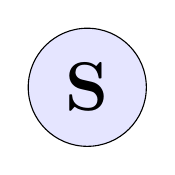
\begin{tikzpicture}
  \node[draw, circle, fill=blue!10, minimum size=1.5cm, font=\bfseries\Huge] {S};
\end{tikzpicture}
\textit{“Is this indivisible?”}
\end{center}
\end{tcolorbox}

Every building needs raw materials.  For Apeiron, the raw material is
something called an \textbf{Ultimate Observable} – a tiny, indivisible
piece of information.  You can think of it as the \emph{quantum} of
experience: the smallest chunk that still carries meaning.

\begin{tcolorbox}[colback=yellow!5, colframe=yellow!80, title=Real‑life analogy]
A 1000‑piece jigsaw puzzle.  You tip the box and a thousand little
cardboard shapes pour out.  Each piece is meaningless by itself, but
together they can become anything.  Apeiron’s Layer~1 is like
carefully picking up one piece, examining it from all sides, and
confirming: \emph{this piece cannot be split further without breaking
the picture it might become.}
\end{tcolorbox}

\textbf{Pixel’s point of view.}
Pixel wakes up and switches on its camera.  It sees a mosaic of tiny
coloured squares – red, blue, green, dark, bright.  That is all it has.
Nobody tells Pixel “this is a rock” or “that is a shadow”.  It just
stares at a sea of numbers.

Pixel asks itself: \emph{is this little square truly basic, or could
I split it into even smaller, still useful pieces?}  If the answer is
“no”, the square becomes an atom – a certified building block of
Pixel’s future knowledge.

\subsection*{Why not just use pixels and be done with it?}

That’s a fair question!  In a digital photo a pixel is already the
smallest dot you can get.  So why go through all the trouble of
inspecting it?  Because Apeiron is not designed only for photos – it
could be fed with sound waves, temperature curves, or the pressure of
a robot’s foot on the ground.  In those worlds, the “smallest
meaningful piece” is not obvious at all.  The four inspectors
guarantee that, whatever the sensor, the system always starts from a
rock‑solid foundation.

\begin{figure}[ht]
\centering
\begin{tikzpicture}[
    checker/.style={rectangle, draw=black, fill=orange!15, minimum width=2.8cm, minimum height=0.7cm, align=center, font=\footnotesize},
    arrow/.style={-{Stealth}, thick}
]
\node (obs) at (0,0) [draw, circle, fill=blue!10] {Pixel (value=192)};
\node (B) at (-3, 2) [checker] {Can I split the number 192? (Boolean)};
\node (M) at (3, 2)  [checker] {Can I cut the pixel area? (Measure)};
\node (C) at (-3, 4) [checker] {Is it the only thing in its group? (Category)};
\node (I) at (3, 4)  [checker] {Can I compress it? (Information)};
\draw[arrow] (obs) -- (B);
\draw[arrow] (obs) -- (M);
\draw[arrow] (B) -- (C);
\draw[arrow] (M) -- (I);
\node at (0,-1.5) {\small If all four say “no”, the pixel is an atom.};
\end{tikzpicture}
\caption{The four mathematical inspectors that certify atomicity.}
\label{fig:atomicity}
\end{figure}

\subsection*{A peek into Pixel’s inspector room}

Imagine Pixel sitting at a desk, a magnifying glass in one hand, a
ruler in the other, a philosophy textbook to the left, and a
compression algorithm on its screen.

\begin{itemize}
    \item The \textbf{Boolean Inspector} mutters: “Hmm, 192 is divisible
    by 2, by 3… but only 1 and itself count.  No proper divisors?  Atom!”
    \item The \textbf{Measure Inspector} measures the pixel area: “If I
    cut this in half, each half still behaves like a pixel?  Yes – so
    it’s safe.”
    \item The \textbf{Category Inspector} looks around: “Is this pixel
    the only one of its kind?  If I delete it, does the whole thing
    collapse?  No?  Then it’s an atom.”
    \item The \textbf{Information Inspector} ZIP‑compresses the pixel:
    “I tried to squeeze it.  It won’t get any smaller.  That means it
    already contains as much info as it can.  Atom!”
\end{itemize}

All four agree.  Pixel stamps the pixel as \textbf{atomic} and stores
it safely in its memory.

% ----- WAT ALS...? -----
\begin{tcolorbox}[colback=orange!5, colframe=orange!60, title=\textbf{What if...?}]
What if the very first atom Pixel picks is actually a meaningless
speck of dust on the camera lens?  Could the whole knowledge tower
collapse because of a dirty sensor?
\end{tcolorbox}